% Section 1.4: from fixed features to learned representations.
\section{Multilayer Perceptrons}
\label{sec:logreg_to_mlp:multilayer_perceptrons}

\subsection{Why add a hidden layer?}
A sigmoid neuron can turn an affine score into a probability, but its $1/2$ decision boundary is still a hyperplane in its input features. If the relationship between those features and the label cannot be separated by a hyperplane, adjusting the sigmoid neuron alone cannot solve the representation problem.

Consider two binary measurements $x_1,x_2$ and a label indicating that exactly one measurement is active:
\[
 (0,0)\mapsto0,\qquad(1,0)\mapsto1,\qquad
 (0,1)\mapsto1,\qquad(1,1)\mapsto0.
\]
This is XOR. To classify it with $\hat y=\mathbf{1}\{w_1x_1+w_2x_2+b\geq0\}$ would require
\[
 b<0,\quad w_1+b\geq0,\quad w_2+b\geq0,\quad w_1+w_2+b<0.
\]
The middle inequalities imply $w_1+w_2+2b\geq0$, hence
$w_1+w_2+b\geq-b>0$, contradicting the last inequality. This is a limitation of the model family, not a failure of an optimizer.

One response is to invent a nonlinear feature, such as $x_1x_2$. Another is to let the model learn features. An MLP does this by composing affine maps and nonlinear activations. Its final sigmoid neuron is logistic regression on the last hidden representation rather than on the raw measurements.
\begin{keyidea}[A hidden layer changes the coordinates used for prediction]
A hidden layer computes $\mathbf{h}(\mathbf{x};\theta)$, a collection of parameterized features. The output model combines those features. Joint learning adjusts both how the input is represented and how the representation is used. A hidden unit is called hidden because it is an internal computation, not an observed target variable.
\end{keyidea}

\subsection{Derive a layer from its individual neurons}
We follow the lecture convention here: inputs are columns, and each neuron's incoming weight vector is a column of $W$. For $k_1$ neurons,
\[
 W^{(1)}=[\mathbf{w}^{(1)}_1\ \cdots\ \mathbf{w}^{(1)}_{k_1}]
 \in\mathbb{R}^{d\times k_1},\qquad
 \mathbf{b}^{(1)}\in\mathbb{R}^{k_1}.
\]
Neuron $j$ computes
\[
 z^{(1)}_j=\sum_{i=1}^d W^{(1)}_{ij}x_i+b^{(1)}_j,
 \qquad h^{(1)}_j=g^{(1)}(z^{(1)}_j).
\]
Stacking these $k_1$ equations gives
\begin{align}
 \underbrace{\mathbf{z}^{(1)}}_{k_1\times1}
 &=\underbrace{W^{(1)\mathsf T}}_{k_1\times d}
   \underbrace{\mathbf{x}}_{d\times1}
   +\underbrace{\mathbf{b}^{(1)}}_{k_1\times1},\\
 \underbrace{\mathbf{h}^{(1)}}_{k_1\times1}
 &=g^{(1)}\!\left(\underbrace{\mathbf{z}^{(1)}}_{k_1\times1}\right).
\end{align}
The activation is applied elementwise and preserves shape. The weights and bias are learned parameters; $\mathbf{z}^{(1)}$ and $\mathbf{h}^{(1)}$ depend on the current example. All neurons in this layer read the same input vector. They do not receive separate examples.

A fully connected layer connects every input coordinate to every output neuron. Consequently it has $dk_1$ weights and $k_1$ biases. The number of connections counts weights, not independent input data points.

\subsection{Compose two hidden layers and an output layer}
Let the output have $c$ coordinates. Set $\mathbf{h}^{(0)}=\mathbf{x}$. Then
\begin{align}
 \mathbf{z}^{(1)}&=W^{(1)\mathsf T}\mathbf{x}+\mathbf{b}^{(1)},
 &\mathbf{h}^{(1)}&=g^{(1)}(\mathbf{z}^{(1)}),\\
 \mathbf{z}^{(2)}&=W^{(2)\mathsf T}\mathbf{h}^{(1)}+\mathbf{b}^{(2)},
 &\mathbf{h}^{(2)}&=g^{(2)}(\mathbf{z}^{(2)}),\\
 \mathbf{z}^{(3)}&=W^{(3)\mathsf T}\mathbf{h}^{(2)}+\mathbf{b}^{(3)},
 &\hat{\mathbf{y}}&=g^{(3)}(\mathbf{z}^{(3)}).
\end{align}
Here $W^{(2)}\in\mathbb{R}^{k_1\times k_2}$ and
$W^{(3)}\in\mathbb{R}^{k_2\times c}$. The output activation depends on the task: a sigmoid for one binary probability, softmax for mutually exclusive classes, or often the identity for unconstrained regression. Hidden activations need not match the output activation.

\begin{figure}[htbp]
\centering
\begin{tikzpicture}[>=Stealth, every node/.style={font=\small},node distance=0.65cm]
\node[draw,rounded corners,align=center] (x) {Input\\$d$ coordinates};
\node[draw,rounded corners,align=center,right=of x] (h1) {Hidden 1\\$k_1$ features};
\node[draw,rounded corners,align=center,right=of h1] (h2) {Hidden 2\\$k_2$ features};
\node[draw,rounded corners,align=center,right=of h2] (y) {Output\\$c$ coordinates};
\draw[->] (x)--(h1); \draw[->] (h1)--(h2); \draw[->] (h2)--(y);
\node[below=0.5cm of h1] {$dk_1$ weights};
\node[below=0.5cm of h2] {$k_1k_2$ weights};
\node[below=0.5cm of y] {$k_2c$ weights};
\end{tikzpicture}
\caption{A forward pass has three affine maps when there are two hidden layers and an output layer. The input is not counted as a computed layer. Each arrow denotes a full matrix transformation followed by an activation.}
\end{figure}

For one hidden layer, the nested form is
\[
 \hat{\mathbf{y}}=g^{(2)}\!\left(W^{(2)\mathsf T}
 g^{(1)}(W^{(1)\mathsf T}\mathbf{x}+\mathbf{b}^{(1)})+\mathbf{b}^{(2)}\right).
\]
The nesting records a dependency: the second layer must wait for the first layer's features. Neurons within a layer can be evaluated together, while successive layers depend on earlier results. A network with only affine maps and elementwise activations also processes different batch examples independently.

\subsection{Why the hidden nonlinearity matters: a proof}
Suppose two consecutive layers have identity activations. Write their affine maps as $A_1\mathbf{x}+\mathbf{b}_1$ and $A_2\mathbf{h}+\mathbf{b}_2$. Substitution gives
\[
 A_2(A_1\mathbf{x}+\mathbf{b}_1)+\mathbf{b}_2
 =\underbrace{A_2A_1}_{A_{\mathrm{eff}}}\mathbf{x}
  +\underbrace{(A_2\mathbf{b}_1+\mathbf{b}_2)}_{\mathbf{b}_{\mathrm{eff}}}.
\]
Induction collapses any finite stack of affine maps into a single affine map. Adding only linear hidden layers therefore cannot solve XOR; with a final sigmoid it is still logistic regression on an affine score. Factorization can affect optimization or impose a rank constraint, but does not produce nonlinear decision geometry.

With $g(z)=\max(0,z)$ (ReLU), each unit can turn off on one side of its own hyperplane. Different inputs activate different subsets of units. Within a fixed activation pattern the map is affine; across patterns it is piecewise affine. This permits several boundary pieces in input space. ReLU is differentiable except at zero, so the slides' differentiability requirement should be read with this common almost-everywhere qualification; learning implementations choose a derivative convention at the kink.

\subsection{A constructive nonlinear representation: solve XOR by hand}
Choose two ReLU features
\[
 h_1=\max(0,x_1-x_2),\qquad
 h_2=\max(0,x_2-x_1).
\]
Their sum is $|x_1-x_2|$. At the four binary inputs:
\begin{center}
\begin{tabular}{ccccc}
\toprule
$(x_1,x_2)$ & $h_1$ & $h_2$ & $h_1+h_2$ & $y$\\
\midrule
$(0,0)$ & 0 & 0 & 0 & 0\\
$(1,0)$ & 1 & 0 & 1 & 1\\
$(0,1)$ & 0 & 1 & 1 & 1\\
$(1,1)$ & 0 & 0 & 0 & 0\\
\bottomrule
\end{tabular}
\end{center}
Now a single output neuron suffices:
\[
 z_{\mathrm{out}}=10(h_1+h_2-0.5),\qquad
 p=\sigma(z_{\mathrm{out}}).
\]
The negative examples have $p=\sigma(-5)\approx0.0067$, and the positive examples have $p=\sigma(5)\approx0.9933$. In hidden space the boundary is the line $h_1+h_2=0.5$. Its preimage in input space is $|x_1-x_2|=0.5$, comprising two parallel lines. The output remains linear in hidden features even though the boundary is not a single line in the original inputs.

\begin{figure}[htbp]
\centering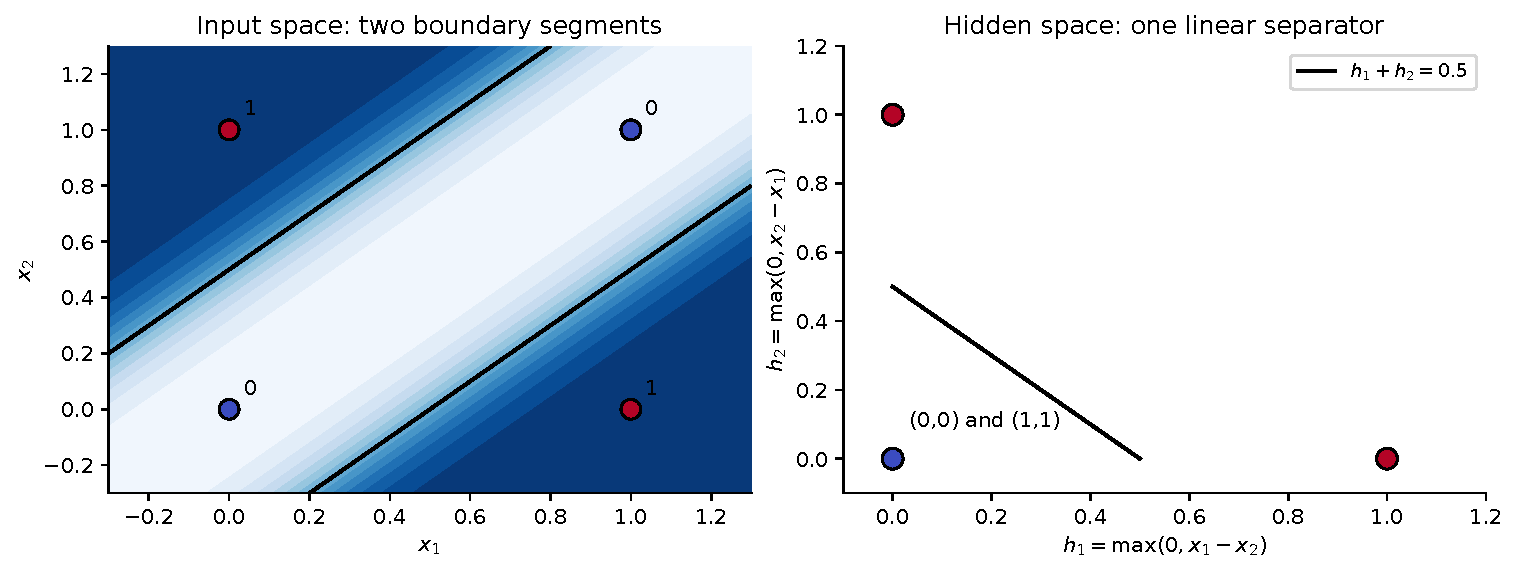
\includegraphics[width=\linewidth]{mlp_1_4_1_5/xor_features.pdf}
\caption{An explicit feature map makes XOR linearly separable. Colors on the left background show the output probability; labeled points are the four binary cases. Both negative examples map to the same hidden point. These features and weights are constructed by hand, demonstrating representability rather than proving a training algorithm will find them.}
\end{figure}

This toy problem has a useful interpretation for perception: two sensors may disagree in a way that predicts a fault, even when either sensor reading alone is uninformative. The learned feature needs to detect a relationship between inputs. Real sensor errors are not literally noiseless XOR, but the example isolates the need for interactions.

Calling hidden units ``adaptable basis functions'' emphasizes this feature-building role. For a scalar output logit,
\[
 z_{\mathrm{out}}=\beta_0+\sum_j\beta_j\phi_j(\mathbf{x};\theta),
\]
where $\phi_j$ are hidden activations. Unlike fixed polynomial features, their parameters can be learned. They need not form a basis in the strict linear-algebra sense: they may be redundant, dependent, or inactive. Also, learning the hidden parameters jointly generally removes logistic regression's convexity guarantee.

\subsection{Time complexity for the lecture's two-hidden-layer question}
Assume dense matrices, ordinary matrix multiplication, fixed-precision scalar arithmetic, and elementwise activations with constant work per coordinate. Standard softmax also takes linear work in its number of output coordinates. Keep $c$ explicit because the question does not specify output width.

For one example, layer 1 multiplies a $k_1\times d$ matrix by a $d\times1$ vector. The hint gives $O(k_1d\cdot1)$. Equivalently, $k_1$ neurons each compute a dot product with $d$ terms. Apply the same argument at the next layers:
\begin{center}
\begin{tabular}{llll}
\toprule
Layer & Matrix product & Product cost & Bias/activation cost\\
\midrule
First hidden & $(k_1\times d)(d\times1)$ & $O(dk_1)$ & $O(k_1)$\\
Second hidden & $(k_2\times k_1)(k_1\times1)$ & $O(k_1k_2)$ & $O(k_2)$\\
Output & $(c\times k_2)(k_2\times1)$ & $O(k_2c)$ & $O(c)$\\
\bottomrule
\end{tabular}
\end{center}
Add sequential work; do not multiply the layer costs together:
\[
 T=O(dk_1+k_1k_2+k_2c+k_1+k_2+c)
   =\boxed{O(dk_1+k_1k_2+k_2c)}.
\]
The last simplification assumes positive integer widths. For a scalar binary output ($c=1$), a useful explicit answer is
\[
 \boxed{T=O(dk_1+k_1k_2+k_2)=O(dk_1+k_1k_2).}
\]
If the intended forward pass stops at the second hidden representation, omit the output-layer term. Writing the architecture next to the answer prevents ambiguity. These counts describe arithmetic work, not exact GPU latency or a promise of ideal parallel speedup.

\subsection{Memory complexity: count what must exist}
Time counts operations; memory counts stored numbers. A multiplication can perform many operations without storing every intermediate scalar product. In the lecture hint, $(n\times m)(m\times k)$ stores two operands and a result, giving $O(nm+mk+nk)$, not $O(nmk)$ storage.

Keep all network parameters resident. The exact number of parameters is
\[
 P=\underbrace{dk_1+k_1k_2+k_2c}_{\text{weights}}
  +\underbrace{k_1+k_2+c}_{\text{biases}}.
\]
The input has $d$ numbers. If all preactivations and activations are retained separately, they use $2(k_1+k_2+c)$ numbers, including the final output. Thus one explicit storage model is
\[
 S_{\mathrm{cache}}=P+d+2(k_1+k_2+c).
\]
An implementation may alias some buffers or save only what a particular activation needs, changing constants. The inclusive big-O answer is
\[
 \boxed{S=O(dk_1+k_1k_2+k_2c+d+k_1+k_2+c).}
\]
For $c=1$ this becomes
\[
 \boxed{S=O(dk_1+k_1k_2+d+k_1+k_2)}.
\]
For positive widths, the product terms dominate these vector terms, so $O(dk_1+k_1k_2)$ is also valid. Showing the unsimplified expression demonstrates that input, output, biases, and intermediate vectors were included as requested.

\begin{warning}[Do not call activation memory the total memory]
$O(d+k_1+k_2+c)$ accounts for input and activations only. It omits the matrices needed to execute the forward pass. Conversely, parameters are stored once, not once per example or once every time they are used. Gradients and optimizer state are separate training allocations and are not required for a forward-only inference calculation.
\end{warning}

For inference, once layer 2 has consumed $\mathbf{h}^{(1)}$, that activation can be released if no later operation needs it. With only two hidden layers, caching versus buffer reuse does not change the order of the vector terms. With variable depth and large batches, the distinction becomes significant; Section~\ref{sec:logreg_to_mlp:matrix_dimensions} makes it explicit.

\subsection{A practical sizing example}
Suppose a grasp-success predictor takes 12 measured features, such as geometric clearance, contact estimates, and pose uncertainty summaries. Choose the illustrative architecture
\[
 12\longrightarrow32\longrightarrow16\longrightarrow1.
\]
It uses $12(32)+32(16)+16(1)=912$ weight multiplications per example, plus the corresponding additions and activations. It has $32+16+1=49$ biases, hence $P=961$ parameters. Retaining input and all $Z/H$ vectors uses
\[
 961+12+2(32+16+1)=1071
\]
scalars. At four bytes per scalar this model accounts for 4,284 bytes. This is an array-element count, not actual process memory: array objects, kernel workspace, allocator overhead, and library code are excluded.

For 256 candidate grasps evaluated together, there are $256(912)=233{,}472$ weight products, while there are still only 961 parameters. The network is reused across candidates. Its predictions would require training and validation before being meaningful; the example here is for architecture and resource accounting.

\subsection{Exercises and worked reasoning}
\paragraph{1. Why does depth without nonlinearity not solve XOR?}
Compose the affine maps including their biases. The result is one affine map, whose threshold is a single hyperplane; the four XOR inequalities remain contradictory. A final sigmoid changes probabilities but not that limitation.

\paragraph{2. What if both hidden widths are doubled?}
For fixed $d,c$, the first-layer products double, the hidden-to-hidden products quadruple, and the output-layer products double. The total factor depends on which term dominates. It is not always exactly four.

\paragraph{3. Is one hidden neuron enough for XOR with ReLU and a sigmoid output?}
No. Its logit is $a\max(0,\mathbf{w}^{\mathsf T}\mathbf{x}+b)+c$, a monotone function of the one affine score (possibly decreasing if $a<0$). Thresholding it gives a half-space, all inputs, or no inputs, with possible boundary ties. XOR requires more than one such half-space decision. The two-unit construction above shows sufficiency.

\paragraph{4. Can a large activation value be interpreted as a probability?}
Not in general. ReLU activations can exceed one, can be rescaled with compensating downstream weights, and need not represent a named semantic concept. The probabilistic interpretation comes from the chosen output distribution and loss, not merely from being a neuron.
